% Created by tikzDevice version 0.12.3.1 on 2022-09-02 16:28:32
% !TEX encoding = UTF-8 Unicode
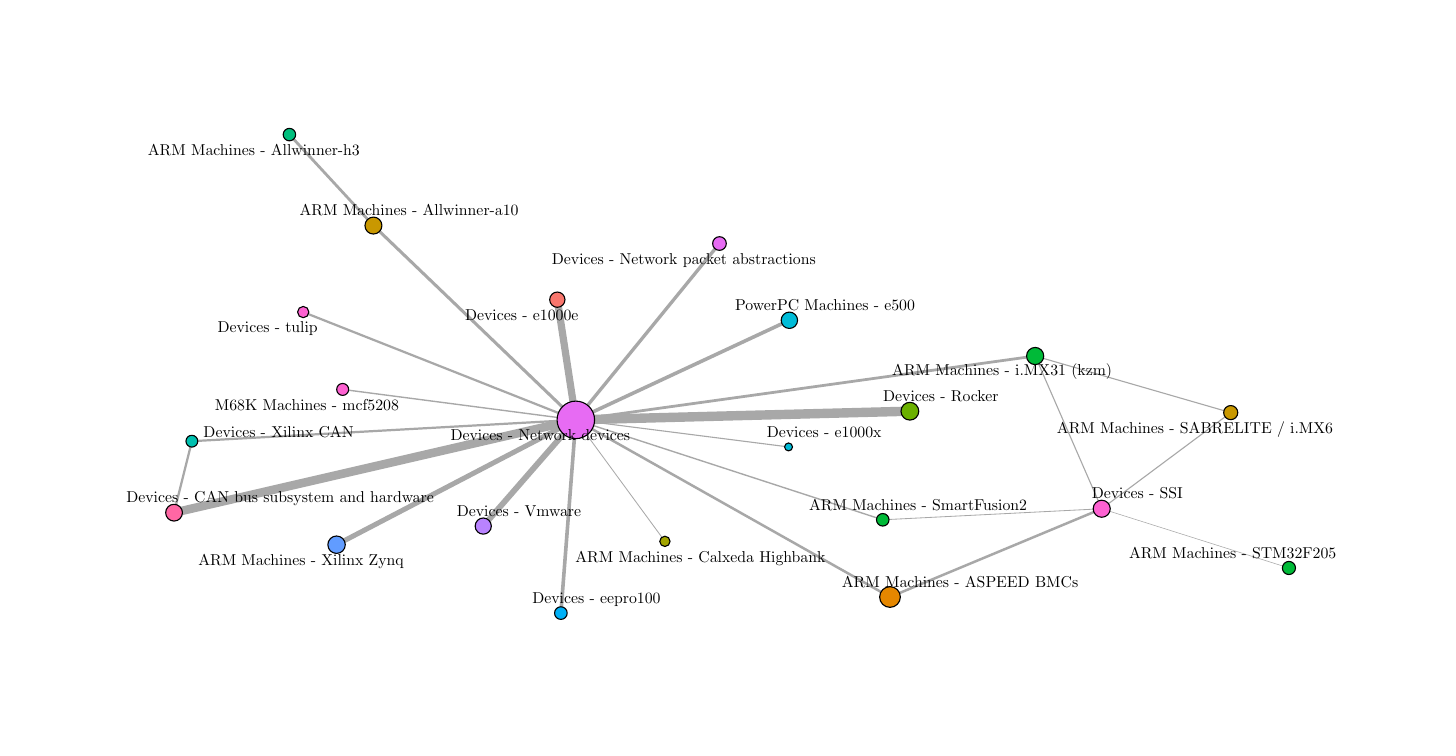
\begin{tikzpicture}[x=1pt,y=1pt]
\definecolor{fillColor}{RGB}{255,255,255}
\path[use as bounding box,fill=fillColor,fill opacity=0.00] (0,0) rectangle (505.89,252.94);
\begin{scope}
\path[clip] (  0.00,  0.00) rectangle (505.89,252.94);
\definecolor{fillColor}{RGB}{255,255,255}

\path[fill=fillColor] (  0.00,  0.00) rectangle (505.89,252.94);
\end{scope}
\begin{scope}
\path[clip] ( 32.75, 32.75) rectangle (475.89,222.94);
\definecolor{drawColor}{gray}{0.66}

\path[draw=drawColor,line width= 0.9pt,line join=round] (311.60, 47.21) -- (198.07,111.22);

\path[draw=drawColor,line width= 0.9pt,line join=round] (311.60, 47.21) -- (388.10, 79.10);

\path[draw=drawColor,line width= 1.0pt,line join=round] (124.94,181.43) -- ( 94.58,214.30);

\path[draw=drawColor,line width= 1.1pt,line join=round] (124.94,181.43) -- (198.07,111.22);

\path[draw=drawColor,line width= 0.3pt,line join=round] (230.26, 67.32) -- (198.07,111.22);

\path[draw=drawColor,line width= 0.4pt,line join=round] (434.72,113.84) -- (364.05,134.29);

\path[draw=drawColor,line width= 0.4pt,line join=round] (434.72,113.84) -- (388.10, 79.10);

\path[draw=drawColor,line width= 0.2pt,line join=round] (455.75, 57.70) -- (388.10, 79.10);

\path[draw=drawColor,line width= 0.5pt,line join=round] (308.98, 75.11) -- (198.07,111.22);

\path[draw=drawColor,line width= 0.3pt,line join=round] (308.98, 75.11) -- (388.10, 79.10);

\path[draw=drawColor,line width= 1.8pt,line join=round] (111.62, 66.11) -- (198.07,111.22);

\path[draw=drawColor,line width= 1.0pt,line join=round] (364.05,134.29) -- (198.07,111.22);

\path[draw=drawColor,line width= 0.4pt,line join=round] (364.05,134.29) -- (388.10, 79.10);

\path[draw=drawColor,line width= 3.1pt,line join=round] ( 52.89, 77.68) -- (198.07,111.22);

\path[draw=drawColor,line width= 0.8pt,line join=round] ( 52.89, 77.68) -- ( 59.33,103.51);

\path[draw=drawColor,line width= 1.2pt,line join=round] (198.07,111.22) -- (249.98,174.94);

\path[draw=drawColor,line width= 3.4pt,line join=round] (198.07,111.22) -- (318.78,114.35);

\path[draw=drawColor,line width= 2.1pt,line join=round] (198.07,111.22) -- (164.62, 72.84);

\path[draw=drawColor,line width= 0.8pt,line join=round] (198.07,111.22) -- ( 59.33,103.51);

\path[draw=drawColor,line width= 2.6pt,line join=round] (198.07,111.22) -- (191.39,154.65);

\path[draw=drawColor,line width= 0.4pt,line join=round] (198.07,111.22) -- (274.94,101.44);

\path[draw=drawColor,line width= 1.3pt,line join=round] (198.07,111.22) -- (192.67, 41.40);

\path[draw=drawColor,line width= 0.8pt,line join=round] (198.07,111.22) -- ( 99.57,150.17);

\path[draw=drawColor,line width= 0.5pt,line join=round] (198.07,111.22) -- (113.82,122.22);

\path[draw=drawColor,line width= 1.3pt,line join=round] (198.07,111.22) -- (275.24,147.21);
\definecolor{drawColor}{RGB}{0,0,0}
\definecolor{fillColor}{RGB}{229,135,0}

\path[draw=drawColor,line width= 0.4pt,line join=round,line cap=round,fill=fillColor] (311.60, 47.21) circle (  3.74);
\definecolor{fillColor}{RGB}{201,152,0}

\path[draw=drawColor,line width= 0.4pt,line join=round,line cap=round,fill=fillColor] (124.94,181.43) circle (  3.06);
\definecolor{fillColor}{RGB}{0,191,125}

\path[draw=drawColor,line width= 0.4pt,line join=round,line cap=round,fill=fillColor] ( 94.58,214.30) circle (  2.25);
\definecolor{fillColor}{RGB}{163,165,0}

\path[draw=drawColor,line width= 0.4pt,line join=round,line cap=round,fill=fillColor] (230.26, 67.32) circle (  1.86);
\definecolor{fillColor}{RGB}{201,152,0}

\path[draw=drawColor,line width= 0.4pt,line join=round,line cap=round,fill=fillColor] (434.72,113.84) circle (  2.55);
\definecolor{fillColor}{RGB}{0,186,56}

\path[draw=drawColor,line width= 0.4pt,line join=round,line cap=round,fill=fillColor] (455.75, 57.70) circle (  2.37);

\path[draw=drawColor,line width= 0.4pt,line join=round,line cap=round,fill=fillColor] (308.98, 75.11) circle (  2.26);
\definecolor{fillColor}{RGB}{97,156,255}

\path[draw=drawColor,line width= 0.4pt,line join=round,line cap=round,fill=fillColor] (111.62, 66.11) circle (  3.15);
\definecolor{fillColor}{RGB}{0,186,56}

\path[draw=drawColor,line width= 0.4pt,line join=round,line cap=round,fill=fillColor] (364.05,134.29) circle (  3.10);
\definecolor{fillColor}{RGB}{255,103,164}

\path[draw=drawColor,line width= 0.4pt,line join=round,line cap=round,fill=fillColor] ( 52.89, 77.68) circle (  3.03);
\definecolor{fillColor}{RGB}{231,107,243}

\path[draw=drawColor,line width= 0.4pt,line join=round,line cap=round,fill=fillColor] (198.07,111.22) circle (  6.78);

\path[draw=drawColor,line width= 0.4pt,line join=round,line cap=round,fill=fillColor] (249.98,174.94) circle (  2.47);
\definecolor{fillColor}{RGB}{107,177,0}

\path[draw=drawColor,line width= 0.4pt,line join=round,line cap=round,fill=fillColor] (318.78,114.35) circle (  3.21);
\definecolor{fillColor}{RGB}{253,97,209}

\path[draw=drawColor,line width= 0.4pt,line join=round,line cap=round,fill=fillColor] (388.10, 79.10) circle (  3.08);
\definecolor{fillColor}{RGB}{185,131,255}

\path[draw=drawColor,line width= 0.4pt,line join=round,line cap=round,fill=fillColor] (164.62, 72.84) circle (  2.92);
\definecolor{fillColor}{RGB}{0,192,175}

\path[draw=drawColor,line width= 0.4pt,line join=round,line cap=round,fill=fillColor] ( 59.33,103.51) circle (  2.13);
\definecolor{fillColor}{RGB}{248,118,109}

\path[draw=drawColor,line width= 0.4pt,line join=round,line cap=round,fill=fillColor] (191.39,154.65) circle (  2.76);
\definecolor{fillColor}{RGB}{0,188,216}

\path[draw=drawColor,line width= 0.4pt,line join=round,line cap=round,fill=fillColor] (274.94,101.44) circle (  1.43);
\definecolor{fillColor}{RGB}{0,176,246}

\path[draw=drawColor,line width= 0.4pt,line join=round,line cap=round,fill=fillColor] (192.67, 41.40) circle (  2.28);
\definecolor{fillColor}{RGB}{253,97,209}

\path[draw=drawColor,line width= 0.4pt,line join=round,line cap=round,fill=fillColor] ( 99.57,150.17) circle (  2.04);

\path[draw=drawColor,line width= 0.4pt,line join=round,line cap=round,fill=fillColor] (113.82,122.22) circle (  2.16);
\definecolor{fillColor}{RGB}{0,188,216}

\path[draw=drawColor,line width= 0.4pt,line join=round,line cap=round,fill=fillColor] (275.24,147.21) circle (  2.96);

\node[text=drawColor,anchor=base,inner sep=0pt, outer sep=0pt, scale=  0.57] at (336.93, 50.78) {ARM Machines - ASPEED BMCs};

\node[text=drawColor,anchor=base,inner sep=0pt, outer sep=0pt, scale=  0.57] at (137.83,185.01) {ARM Machines - Allwinner-a10};

\node[text=drawColor,anchor=base,inner sep=0pt, outer sep=0pt, scale=  0.57] at ( 81.74,206.82) {ARM Machines - Allwinner-h3};

\node[text=drawColor,anchor=base,inner sep=0pt, outer sep=0pt, scale=  0.57] at (243.10, 59.86) {ARM Machines - Calxeda Highbank};

\node[text=drawColor,anchor=base,inner sep=0pt, outer sep=0pt, scale=  0.57] at (421.82,106.35) {ARM Machines - SABRELITE / i.MX6};

\node[text=drawColor,anchor=base,inner sep=0pt, outer sep=0pt, scale=  0.57] at (435.44, 61.27) {ARM Machines - STM32F205};

\node[text=drawColor,anchor=base,inner sep=0pt, outer sep=0pt, scale=  0.57] at (321.76, 78.64) {ARM Machines - SmartFusion2};

\node[text=drawColor,anchor=base,inner sep=0pt, outer sep=0pt, scale=  0.57] at ( 98.77, 58.61) {ARM Machines - Xilinx Zynq};

\node[text=drawColor,anchor=base,inner sep=0pt, outer sep=0pt, scale=  0.57] at (352.12,127.25) {ARM Machines - i.MX31 (kzm)};

\node[text=drawColor,anchor=base,inner sep=0pt, outer sep=0pt, scale=  0.57] at ( 91.21, 81.22) {Devices - CAN bus subsystem and hardware};

\node[text=drawColor,anchor=base,inner sep=0pt, outer sep=0pt, scale=  0.57] at (185.25,103.76) {Devices - Network devices};

\node[text=drawColor,anchor=base,inner sep=0pt, outer sep=0pt, scale=  0.57] at (237.10,167.48) {Devices - Network packet abstractions};

\node[text=drawColor,anchor=base,inner sep=0pt, outer sep=0pt, scale=  0.57] at (329.97,117.69) {Devices - Rocker};

\node[text=drawColor,anchor=base,inner sep=0pt, outer sep=0pt, scale=  0.57] at (400.97, 82.66) {Devices - SSI};

\node[text=drawColor,anchor=base,inner sep=0pt, outer sep=0pt, scale=  0.57] at (177.52, 76.40) {Devices - Vmware};

\node[text=drawColor,anchor=base,inner sep=0pt, outer sep=0pt, scale=  0.57] at ( 90.66,104.76) {Devices - Xilinx CAN};

\node[text=drawColor,anchor=base,inner sep=0pt, outer sep=0pt, scale=  0.57] at (178.54,147.16) {Devices - e1000e};

\node[text=drawColor,anchor=base,inner sep=0pt, outer sep=0pt, scale=  0.57] at (287.81,105.01) {Devices - e1000x};

\node[text=drawColor,anchor=base,inner sep=0pt, outer sep=0pt, scale=  0.57] at (205.52, 44.96) {Devices - eepro100};

\node[text=drawColor,anchor=base,inner sep=0pt, outer sep=0pt, scale=  0.57] at ( 86.70,142.69) {Devices - tulip};

\node[text=drawColor,anchor=base,inner sep=0pt, outer sep=0pt, scale=  0.57] at (100.91,114.72) {M68K Machines - mcf5208};

\node[text=drawColor,anchor=base,inner sep=0pt, outer sep=0pt, scale=  0.57] at (288.14,150.79) {PowerPC Machines - e500};
\end{scope}
\end{tikzpicture}
